\documentclass[10pt,twocolumn]{article}

\usepackage[letterpaper,margin=0.70in,columnsep=0.22in]{geometry}
\usepackage{amsmath,amssymb}
\usepackage{graphicx}
\usepackage{booktabs}
\usepackage{array}
\usepackage{url}
\usepackage[colorlinks=true,linkcolor=black,citecolor=black,urlcolor=black]{hyperref}

\graphicspath{{../../}{../../results/}{../../reports/}}
\setlength{\parindent}{1em}
\setlength{\parskip}{0pt}
\setlength{\textfloatsep}{8pt plus 2pt minus 2pt}
\setlength{\floatsep}{7pt plus 2pt minus 2pt}
\setlength{\intextsep}{7pt plus 2pt minus 2pt}
\renewcommand{\arraystretch}{1.08}
\emergencystretch=2em
\frenchspacing
\raggedbottom

\newcommand{\vect}[1]{\mathbf{#1}}
\newcommand{\mat}[1]{\mathbf{#1}}
\newcommand{\unit}[1]{\hat{\mathbf{#1}}}
\newcommand{\LU}{\mathrm{LU}}
\newcommand{\TU}{\mathrm{TU}}
\newcommand{\ND}{\mathrm{ND}}
\newcommand{\CRTBP}{CR3BP}
\newcommand{\chisq}{\chi^2}

\title{\vspace{-0.35in}Bearing-Only Optical Navigation and Midcourse Correction in Cislunar Space}
\author{Varsha Krishnakumar\\ASTE 581: Orbital Mechanics II}
\date{Final Project Report}

\begin{document}

\twocolumn[
\begin{@twocolumnfalse}
\maketitle
\vspace{-0.15in}
\begin{abstract}
This report develops and evaluates an end-to-end optical navigation pipeline for a representative cislunar arc in the Earth and Moon system.  A simulated spacecraft observes the Moon with a calibrated pinhole camera, converts noisy pixel centroids into line-of-sight bearings, estimates its six-state position and velocity with an iterated extended Kalman filter (IEKF), and computes an autonomous single-impulse midcourse correction from the estimated state.  The key question is not only whether bearing-only measurements can reduce state error, but whether the resulting estimate is accurate and statistically credible enough to support guidance.  The project couples Circular Restricted Three-Body Problem (CR3BP) dynamics, state-transition-matrix covariance propagation, tangent-plane bearing residuals, pixel-level measurement simulation, active camera pointing, Monte Carlo robustness analysis, and preliminary feature-tracking experiments.  In the final tuned baseline, 1000 Monte Carlo trials with $\sigma_{\rm px}=1$ pixel achieved a median terminal miss of $1.81\times10^{-4}$ nondimensional length units ($70.6$ km using the JPL Earth and Moon length scale), a $99.1\%$ success rate for a $10^{-3}$ length-unit miss tolerance, and a median relative $\Delta V$ inflation of $1.19\%$ relative to the perfect-information burn.  The same run had median NIS $1.94$ for a two-dimensional bearing residual and $99.4\%$ of trial-mean NEES values inside the $\chisq(6)$ 95\% interval.  Active pointing was essential: fixed pointing kept the target visible for only $24.6\%$ of the arc, while estimate-driven pointing maintained $99.7\%$ visibility and kept the estimator stable.
\end{abstract}
\vspace{0.12in}
\end{@twocolumnfalse}
]

\section*{Nomenclature}
\begin{tabular}{@{}p{0.18\linewidth}p{0.74\linewidth}@{}}
$\vect{x}$ & spacecraft state, $[\vect{r}^T,\vect{v}^T]^T\in\mathbb{R}^6$ \\
$\mu$ & CR3BP mass parameter for the Earth and Moon system \\
$\Phi(t,t_0)$ & state transition matrix (STM) \\
$\vect{P}$ & state-estimation covariance \\
$\vect{Q}_d$ & discrete process-noise covariance \\
$q_a$ & white-acceleration process-noise spectral density \\
$\unit{u}$ & line-of-sight (LOS) unit vector \\
$\vect{E}$ & tangent-plane projection basis for bearing residuals \\
$\vect{H}$ & measurement sensitivity matrix \\
$\vect{R}$ & bearing measurement-noise covariance \\
$\vect{K}$ & Kalman gain \\
$t_c$ & correction-burn time \\
NIS & normalized innovation squared \\
NEES & normalized estimation error squared \\
LU, TU & CR3BP nondimensional length and time units \\
\end{tabular}

\section{Introduction}
Future cislunar missions will operate in a regime where ground tracking is valuable but not always sufficient as the only navigation source.  Line-of-sight access can be intermittent, antenna resources are shared, and the geometry of the Earth and Moon system can make updates sparse near operationally sensitive phases.  A camera is attractive because it is passive, lightweight, and already present on many spacecraft for inspection, landing, or science.  The limitation is equally important: a single image of a body gives direction, not range.  Bearing-only optical navigation therefore succeeds only if the dynamics and changing observation geometry supply enough information to recover the missing depth state.

The purpose of this project is to test that idea in a closed-loop cislunar setting.  The contribution is not a new estimator theory result; it is a software and analysis pipeline that connects pixel-level optical measurements to a guidance-relevant endpoint: the quality of a midcourse correction burn.  The core hypothesis is:
\begin{quote}
Bearing measurements, when fused with nonlinear cislunar dynamics and protected by active pointing, can produce state estimates accurate enough to compute near-benchmark correction maneuvers.
\end{quote}
The project began with idealized CR3BP propagation and bearing updates, then progressively added pixel projection, field-of-view gating, process-noise tuning, Monte Carlo uncertainty, and estimate-driven camera re-pointing.  The primary contribution is a systems-level analysis of bearing-only optical navigation in a cislunar environment carried through to a guidance-relevant outcome.  Unlike prior work that relies on position-producing image processing, radiometric range/Doppler, or multiple-body triangulation, this study isolates the minimal case of direction-only measurements and examines how observability emerges through nonlinear dynamics, measurement geometry, and active measurement availability.  To the author's knowledge, this is one of the first studies to explicitly couple bearing-only observability, active pointing policy, and midcourse correction performance in a unified cislunar navigation analysis.

\begin{figure}[t]
\centering
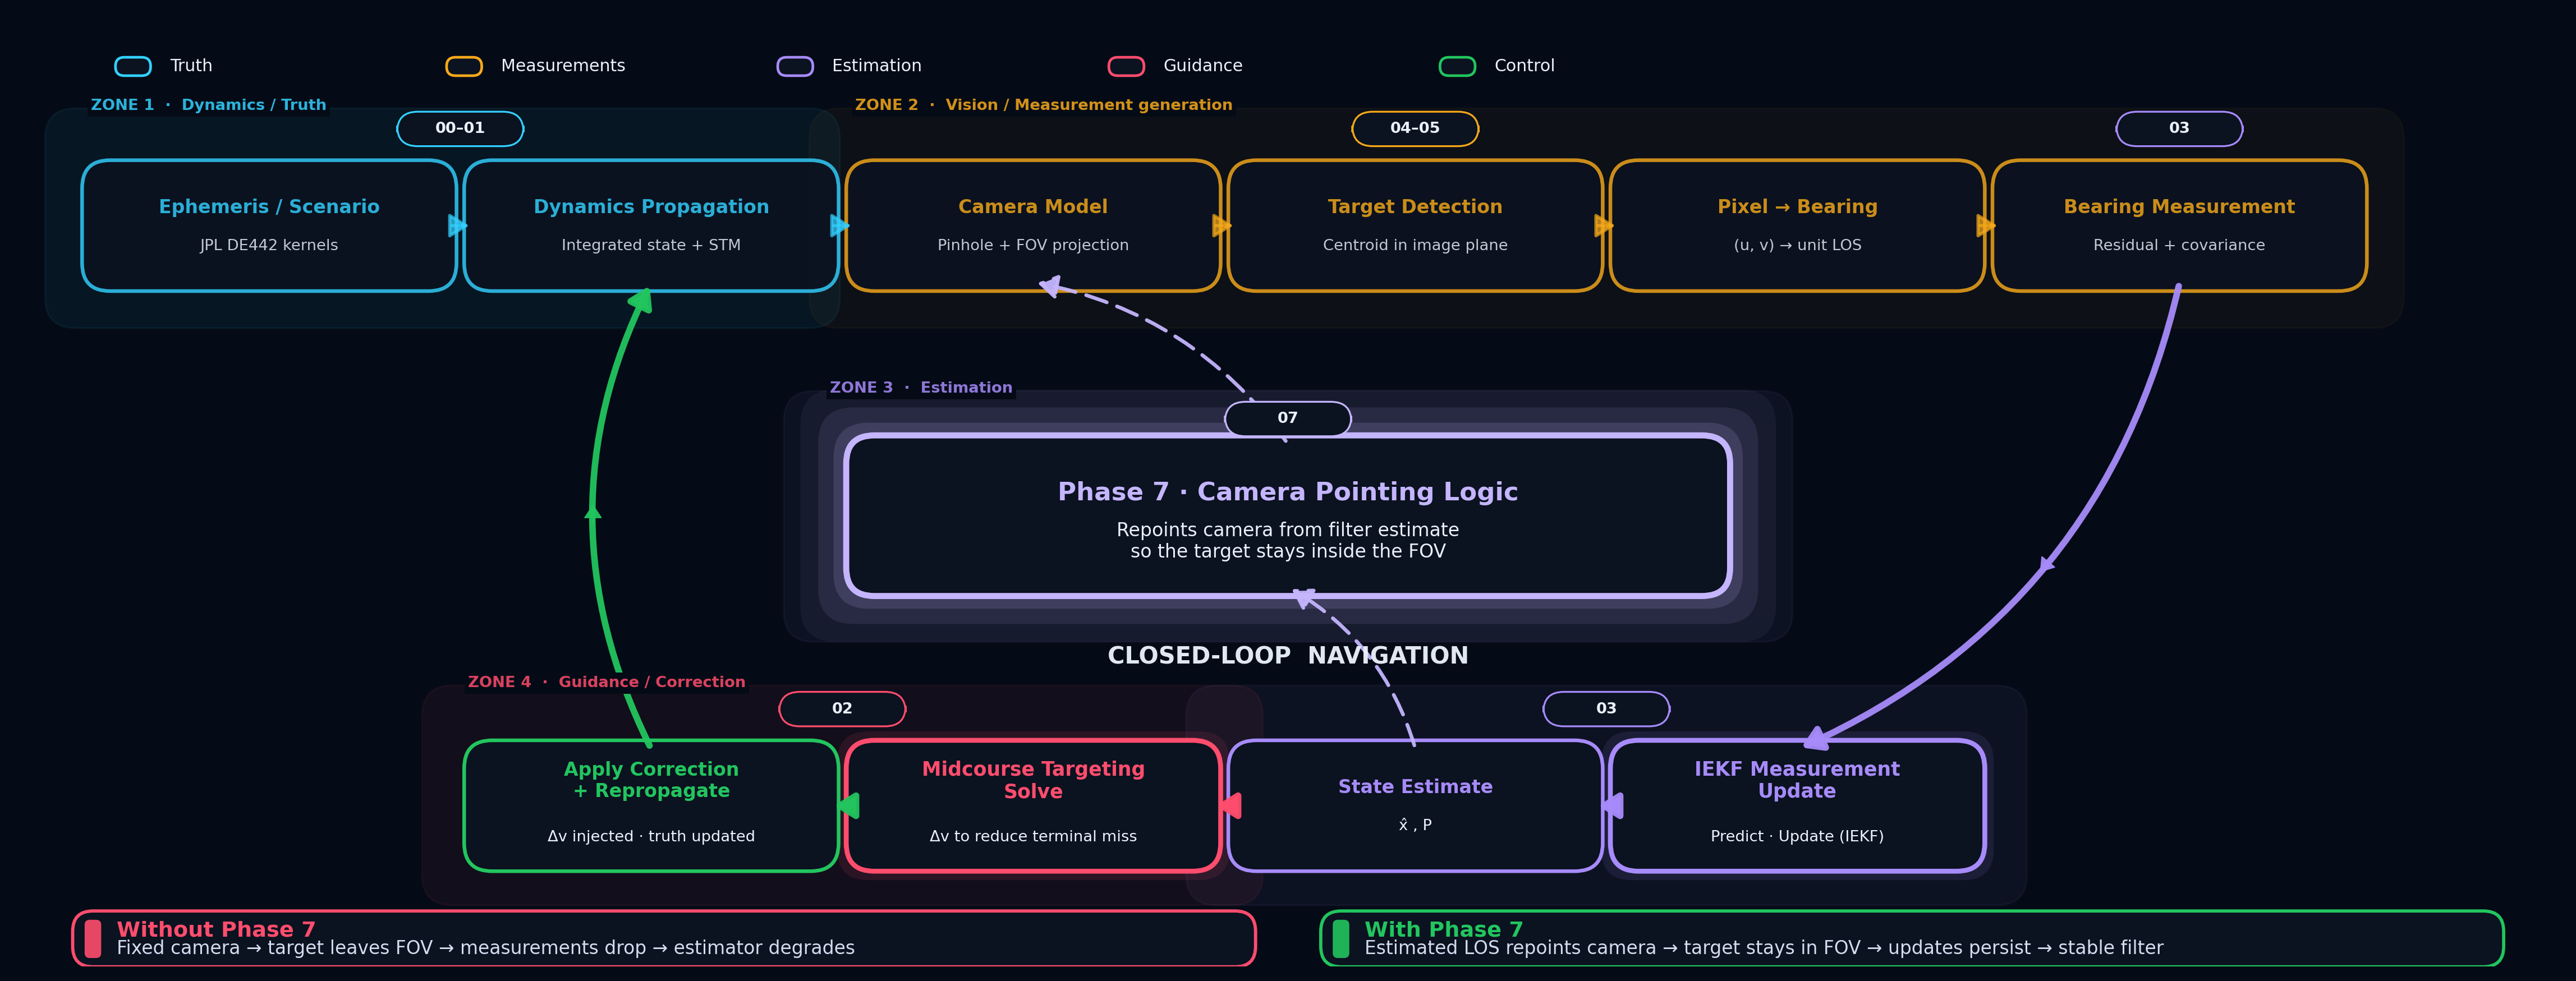
\includegraphics[width=\linewidth]{../../reports/pipeline_diagram.png}
\caption{Closed-loop software architecture used in the project.  The truth model generates the cislunar trajectory, the camera model generates pixel observations, the IEKF produces the navigation state, targeting computes the midcourse burn, and active pointing closes the measurement-availability loop.}
\label{fig:pipeline}
\end{figure}

\section{Comparison to Existing Work}
Optical navigation has been widely studied in both planetary and cislunar contexts, but the measurement products differ substantially across the literature.  Horizon- or limb-based methods use the apparent conic of an extended body to estimate position, attitude, or both; Christian's tutorial gives a complete treatment of that class of algorithms~\cite{christian2021}.  Cislunar navigation studies have also considered natural and artificial optical targets, lunar landmarks, and horizon-based measurements in multi-sensor or higher-fidelity settings~\cite{bradley2020,hinga2023}.  Operational deep-space navigation often combines optical plane-of-sky information with radiometric tracking, where range and Doppler directly improve line-of-sight observability~\cite{ely2021}.  Recent flight demonstrations such as LONEStar further show the value of optical triangulation with multiple planetary targets~\cite{krause2024}.

This report intentionally removes several of those information sources.  The simulated sensor does not fit a lunar limb, track a known landmark in the filter, use radiometric range/Doppler, or triangulate against multiple planets.  It uses a Moon-center bearing derived from pixel centroids, so each accepted frame contributes only two angular constraints.  While a direct numerical comparison is not strictly one-to-one because the measurement models differ, the results here provide a lower bound on performance achievable with minimal-information sensing.

\section{Mission Scenario}
The nominal scenario is a southern halo/near-rectilinear halo orbit (NRHO)-class arc near the Earth and Moon $L_2$ region, seeded from the JPL periodic-orbits catalog and visualized with SPICE-backed ephemeris data.  The cached catalog record in the repository identifies the Earth and Moon system with
\[
\mu=1.215058560962404\times10^{-2},
\]
\[
1\,\LU=389703.2648\ \mathrm{km},
\]
and
\[
1\,\TU=382981.2891\ \mathrm{s}=4.4327\ \mathrm{days}.
\]
Most navigation and targeting results are reported in nondimensional CR3BP units.  The final Monte Carlo tolerance of $10^{-3}\,\LU$ therefore corresponds to approximately $390$ km.  The project slide deck frames the representative arc as a $6.56$ day cislunar tracking window with an insertion/tracking phase and a midcourse correction event.

The numbered scripts implement a staged build-up.  Script \texttt{00} fetches and caches periodic-orbit seeds; \texttt{01} bridges the seed into a SPICE-backed propagation product; scripts \texttt{02} through \texttt{05} develop targeting, ideal bearings, pixel bearings, and camera-feed simulation; \texttt{06} adds IEKF-guided midcourse correction, diagnostics, sensitivity, Monte Carlo, and process-noise tuning; \texttt{07} adds active pointing; and \texttt{08} previews feature tracking.  The codebase deliberately separates reusable models under \texttt{src/} from experiment scripts under \texttt{scripts/}.

\begin{figure}[t]
\centering
\includegraphics[width=\linewidth]{../../results/seeds/spice_nrho_seed.png}
\caption{SPICE-backed seed visualization used to ground the project in a cislunar orbit geometry.  The estimator and guidance studies use nondimensional CR3BP states, while this product keeps the scenario interpretable in the physical geometry of the Earth and Moon system.}
\label{fig:seed}
\end{figure}

\section{Dynamics and Propagation}
\subsection{CR3BP Model}
The primary filter and targeting experiments use the CR3BP for the Earth and Moon system in the synodic frame.  The primaries are fixed at
\[
\vect{r}_E=(-\mu,0,0)^T,\qquad \vect{r}_M=(1-\mu,0,0)^T.
\]
For spacecraft position $(x,y,z)$,
\begin{align}
r_1 &= \sqrt{(x+\mu)^2+y^2+z^2},\\
r_2 &= \sqrt{(x-1+\mu)^2+y^2+z^2},
\end{align}
and the pseudo-potential is
\begin{equation}
\Omega(x,y,z)=\frac{1}{2}(x^2+y^2)+\frac{1-\mu}{r_1}+\frac{\mu}{r_2}.
\end{equation}
The implemented equations of motion are
\begin{align}
\dot{x} &= v_x, & \dot{y} &= v_y, & \dot{z} &= v_z,\\
\dot{v}_x &= 2v_y+\Omega_x, &
\dot{v}_y &= -2v_x+\Omega_y, &
\dot{v}_z &= \Omega_z.
\end{align}
The same \texttt{CR3BP} class also computes the Jacobi constant, the Hessian of $\Omega$, the linearized dynamics matrix $\mat{A}$, and the collinear/triangular Lagrange points.  This gives the estimator both a nonlinear propagation model and the variational dynamics needed for covariance transport.

\subsection{State Transition Matrix}
Covariance propagation uses the STM,
\[
\Phi(t,t_0)=\frac{\partial \vect{x}(t)}{\partial \vect{x}(t_0)}.
\]
The state and STM are propagated together through
\begin{equation}
\dot{\Phi}(t,t_0)=\mat{A}(t)\Phi(t,t_0), \qquad \Phi(t_0,t_0)=\mat{I}_6.
\end{equation}
In implementation, the state and column-major STM are packed into a 42-element vector.  The filter step integrates this combined system with adaptive tolerances, unpacks the terminal state and STM, and updates covariance as
\begin{equation}
\bar{\vect{P}}_{k+1}
 = \Phi_k\vect{P}_k^+\Phi_k^T+\vect{Q}_{d,k}.
\end{equation}
Small numerical asymmetries are removed by symmetrizing $\vect{P}$.  A positive-definiteness guard distinguishes harmless roundoff from true divergence.

\subsection{Process Noise}
The process-noise model is discrete white acceleration on the six-state vector:
\begin{equation}
\vect{Q}_d(\Delta t)=q_a
\begin{bmatrix}
\frac{\Delta t^3}{3}\mat{I}_3 & \frac{\Delta t^2}{2}\mat{I}_3\\
\frac{\Delta t^2}{2}\mat{I}_3 & \Delta t\mat{I}_3
\end{bmatrix}.
\label{eq:q}
\end{equation}
This model is intentionally simple: it represents unmodeled accelerations, numerical/model mismatch, and the covariance inflation required to keep the filter honest.  The final tuning study shows why this matters.  Very small $q_a$ values can produce accurate-looking point estimates while under-reporting uncertainty, which appears as excessive NEES.

\section{Optical Measurement Model}
\subsection{Pixel to Bearing}
The camera is modeled with pinhole intrinsics
\[
\mat{K} =
\begin{bmatrix}
f_x & 0 & c_x\\
0 & f_y & c_y\\
0 & 0 & 1
\end{bmatrix}.
\]
For a pixel detection $(u_{\rm px},v_{\rm px})$, the normalized camera-frame ray is
\begin{equation}
\unit{u}_{C}=
\frac{[(u_{\rm px}-c_x)/f_x,\ (v_{\rm px}-c_y)/f_y,\ 1]^T}
{\left\|[(u_{\rm px}-c_x)/f_x,\ (v_{\rm px}-c_y)/f_y,\ 1]^T\right\|}.
\end{equation}
The ray is rotated into the navigation frame using the current camera attitude.  A scalar pixel standard deviation is converted to angular noise using
\begin{equation}
\sigma_\theta \approx \frac{\sigma_{\rm px}}{f_x},
\end{equation}
or a root-mean-square focal-length variant when $f_x\neq f_y$.  The result is a noisy unit LOS vector and a two-dimensional angular covariance for the bearing residual.

The measurement simulator includes Gaussian pixel noise, optional random dropout, field-of-view clipping, behind-camera rejection, simple distortion hooks, and bounding-box body measurements.  These effects are sufficient to connect camera geometry to the estimator without claiming a flight image-processing pipeline.

\subsection{Tangent-Plane Residual}
Let $\vect{r}_{sc}$ be the spacecraft position and $\vect{r}_b$ be the observed body position, usually the Moon.  The predicted LOS is
\begin{equation}
\unit{u}(\vect{x})=
\frac{\vect{r}_b-\vect{r}_{sc}}
{\left\|\vect{r}_b-\vect{r}_{sc}\right\|}.
\end{equation}
Using all three components of a unit vector would introduce a redundant constraint because $\|\unit{u}\|=1$.  The implementation instead forms an orthonormal tangent basis $\vect{e}_1,\vect{e}_2$ perpendicular to the predicted LOS and stacks it as
\[
\mat{E}=\begin{bmatrix}\vect{e}_1^T\\\vect{e}_2^T\end{bmatrix}.
\]
The two-dimensional innovation is
\begin{equation}
\vect{y}_k = \mat{E}\left(\unit{u}_{\rm meas}-\unit{u}(\bar{\vect{x}}_k)\right).
\label{eq:resid}
\end{equation}
For range $\rho=\|\vect{r}_b-\vect{r}_{sc}\|$, the LOS position sensitivity is
\begin{equation}
\frac{\partial \unit{u}}{\partial \vect{r}_{sc}}
=-\frac{1}{\rho}\left(\mat{I}_3-\unit{u}\unit{u}^T\right),
\end{equation}
giving the measurement matrix
\begin{equation}
\mat{H}=
\begin{bmatrix}
\mat{E}\frac{\partial \unit{u}}{\partial \vect{r}_{sc}} & \mat{0}_{2\times3}
\end{bmatrix},
\qquad
\mat{R}=\sigma_\theta^2\mat{I}_2.
\label{eq:h-bearing}
\end{equation}
This is the mathematical center of the bearing-only estimator: one image contributes two angular constraints, and the range direction must be recovered over time through motion and dynamics.

\begin{figure}[t]
\centering
\includegraphics[width=\linewidth]{../../results/demos/04_pixel_bearings_report.png}
\caption{Pixel-bearing demonstration.  The pipeline projects the target into the image plane, adds pixel-level uncertainty, converts the detection back into a unit LOS vector, and updates the bearing-only filter.}
\label{fig:pixel}
\end{figure}

\section{Bearing-Only Observability}
\subsection{Instantaneous Rank}
At a single image time, the tangent-plane bearing measurement is rank deficient by construction.  The matrix in Eq.~\eqref{eq:h-bearing} has rank at most two because the measurement lives in the plane normal to the predicted LOS:
\begin{equation}
\mathrm{rank}(\mat{H}_k)\le 2.
\end{equation}
For position alone, this is the familiar ``missing range'' intuition: if the observed body location is known and the bearing direction is known, the spacecraft position lies somewhere on a line.  For the full six-state problem, the instantaneous nullspace is larger because the measurement has no direct velocity sensitivity.  One accepted frame leaves the LOS/range position direction and all three velocity directions unconstrained at that instant.  Velocity and range only become observable through the time history of CR3BP motion and the way later LOS measurements depend on earlier position and velocity through the STM.

Over an arc, the relevant local observability object is the stacked linearized measurement history
\begin{equation}
\mathcal{O}_N =
\begin{bmatrix}
\mat{H}_1\Phi(t_1,t_0)\\
\mat{H}_2\Phi(t_2,t_0)\\
\vdots\\
\mat{H}_N\Phi(t_N,t_0)
\end{bmatrix}.
\end{equation}
Equivalently, the diagnostic script accumulates the unweighted Gramian
\begin{equation}
\mat{W}_N=\sum_{k=1}^{N}
\Phi(t_k,t_0)^T\mat{H}_k^T\mat{H}_k\Phi(t_k,t_0),
\label{eq:gramian}
\end{equation}
with a noise-weighted version obtained by inserting $\mat{R}_k^{-1}$ between $\mat{H}_k^T$ and $\mat{H}_k$.  Full rank of $\mat{W}_N$ is a necessary local test, but its conditioning is the more practical metric: a full-rank Gramian can still contain a very weak direction that makes range or velocity slow to recover.  In practice, these weak directions correspond primarily to range and to certain velocity components aligned with the line of sight.

\subsection{Geometry Loss Cases}
The measurement history loses practical observability when the LOS direction changes too little, when the relative motion is nearly straight-line over the tracking window, or when the STM does not couple velocity errors into later angular errors strongly enough before the correction time.  It also loses observability operationally when pointing or field-of-view limits remove measurements, even if the mathematical trajectory would otherwise be informative.  This explains why early correction times and fixed pointing are fragile in the results: the filter either has not yet accumulated enough angular parallax or has been starved of updates.

Figure~\ref{fig:observability} is the direct observability diagnostic generated by \texttt{scripts/06\_midcourse\_ekf\_correction.py}.  In the estimate-tracking case, all six Gramian eigenvalues grow before the correction time, but the final condition number is still $2.90\times10^{6}$.  The weakest direction is therefore not exactly unobservable; it is simply much less informed than the dominant directions.  This is the analytical version of the qualitative statement that range becomes recoverable over time: changing LOS geometry and nonlinear dynamics gradually rotate angular information into the missing state directions.

\begin{figure*}[t]
\centering
\includegraphics[width=0.94\textwidth]{../../results/mc/single_trial/06_observability.png}
\caption{Bearing-only observability diagnostic for a representative estimate-tracking run.  The accumulated Gramian is full rank by the correction time, but its eigenvalue spread remains large, confirming that some range/velocity combinations are only weakly informed.  The rolling acceptance panel also shows why observability is inseparable from measurement availability.}
\label{fig:observability}
\end{figure*}

\section{Estimator}
\subsection{Iterated EKF}
The IEKF prediction is the STM propagation described above.  The measurement update uses the standard innovation covariance
\[
\mat{S}_k=\mat{H}_k\bar{\vect{P}}_k\mat{H}_k^T+\mat{R}_k
\]
and Kalman gain
\[
\mat{K}_k=\bar{\vect{P}}_k\mat{H}_k^T\mat{S}_k^{-1}.
\]
Because the bearing measurement is nonlinear in position, the correction is iterated.  With prior state $\bar{\vect{x}}$ and iteration state $\vect{x}^{(i)}$, the implemented correction has the form
\begin{equation}
\vect{x}^{(i+1)}
=\bar{\vect{x}}
+\mat{K}^{(i)}
\left[
\vect{y}^{(i)}
+\mat{H}^{(i)}\left(\vect{x}^{(i)}-\bar{\vect{x}}\right)
\right].
\end{equation}
The covariance is then updated with the Joseph form,
\begin{equation}
\vect{P}^{+}=(\mat{I}-\mat{K}\mat{H})\bar{\vect{P}}
(\mat{I}-\mat{K}\mat{H})^T+\mat{K}\mat{R}\mat{K}^T,
\end{equation}
which is more robust to numerical loss of symmetry and positive definiteness than the simplified update.

\subsection{Statistical Health Metrics}
The estimator is evaluated with both measurement-space and state-space consistency tests.  The normalized innovation squared is
\begin{equation}
\mathrm{NIS}_k = \vect{y}_k^T\mat{S}_k^{-1}\vect{y}_k.
\end{equation}
For the two-dimensional tangent-plane residual, NIS should be distributed like $\chisq(2)$ under correct modeling.  The normalized estimation error squared is
\begin{equation}
\mathrm{NEES}_k=(\hat{\vect{x}}_k-\vect{x}_k)^T
\vect{P}_k^{-1}(\hat{\vect{x}}_k-\vect{x}_k),
\end{equation}
which is compared to $\chisq(6)$ for the six-state estimate.  The diagnostics suite also plots innovation histories, visibility gating, position/velocity $3\sigma$ envelopes, image-plane detections, and hypothesis checks.

\begin{figure*}[t]
\centering
\includegraphics[width=0.94\textwidth]{../../results/diagnostics/06_ekf/estimate_tracking_baseline/plots/dashboard.png}
\caption{Representative diagnostic dashboard for estimate-tracking.  The diagnostic products connect state error, covariance, innovation consistency, and measurement availability in one run, making filter failures traceable instead of anecdotal.}
\label{fig:dashboard}
\end{figure*}

\section{Guidance Coupling}
The guidance problem asks whether the estimated state is good enough to compute a useful midcourse correction.  A single impulsive burn is applied at correction time $t_c$.  For a candidate burn $\Delta\vect{v}$, the state at $t_c$ is modified as
\[
\vect{x}_{c}^{+}=
\begin{bmatrix}
\vect{r}_c\\
\vect{v}_c+\Delta\vect{v}
\end{bmatrix}.
\]
The targeting routine propagates from $t_c$ to $t_f$ with the STM and solves for a burn that drives the terminal position toward a desired target position.  Linearizing the terminal position with respect to the burn gives
\begin{equation}
\delta\vect{r}_f \approx \Phi_{rv}(t_f,t_c)\,\delta\vect{v}_c,
\end{equation}
where $\Phi_{rv}$ is the upper-right $3\times3$ block of the STM from correction time to final time.  Newton iterations update
\begin{equation}
\Delta\vect{v}_{j+1}
=\Delta\vect{v}_{j}
-\Phi_{rv}^{-1}\left(\vect{r}_{f,j}-\vect{r}_{\rm target}\right),
\end{equation}
using a least-squares fallback if the block is ill-conditioned.  Three cases are compared: no correction, perfect-information correction from the true state, and IEKF correction from the estimated state.

\begin{figure}[t]
\centering
\includegraphics[width=\linewidth]{../../results/mc/single_trial/06_midcourse_report.png}
\caption{Single-trial midcourse correction report.  The IEKF-fed correction is compared against a perfect-information correction and an uncorrected trajectory, making the navigation error visible as guidance performance.}
\label{fig:midcourse}
\end{figure}

\section{Active Camera Pointing}
\subsection{Policy}
Fixed body pointing is a fragile assumption in cislunar optical navigation.  If the Moon drifts out of frame, measurements disappear and the filter reverts to open-loop propagation in a strongly nonlinear dynamical environment.  The active pointing policy therefore treats camera orientation as part of the navigation architecture.  At each measurement epoch, the current state estimate and target position define a desired LOS,
\[
\unit{b}_{\rm cmd}=
\frac{\vect{r}_b-\hat{\vect{r}}_{sc}}
{\|\vect{r}_b-\hat{\vect{r}}_{sc}\|}.
\]
The camera direction-cosine matrix is rebuilt so that the camera boresight aligns with this commanded LOS while an ``up'' hint resolves roll.  The simulator then projects the true target into that camera frame.  This closes the loop:
\[
\hat{\vect{x}}\rightarrow \mathrm{camera\ attitude}
\rightarrow \mathrm{pixels}\rightarrow \mathrm{bearing}
\rightarrow \hat{\vect{x}}.
\]

\subsection{Effect on Observability}
Table~\ref{tab:active} shows the effect.  The fixed camera only preserves visibility for $24.6\%$ of the 301 measurement epochs; active pointing preserves $99.7\%$.  The fixed case eventually diverges because the filter stops receiving useful measurements, while active pointing holds the target near the principal point and keeps the estimator stable.

\begin{table}[t]
\centering
\caption{Fixed versus estimate-driven active pointing on the 301-step active-tracking experiment.  Errors are in nondimensional CR3BP units.}
\label{tab:active}
\footnotesize
\begin{tabular}{@{}lcc@{}}
\toprule
Metric & Fixed & Active \\
\midrule
Visibility fraction & 0.2458 & 0.9967 \\
Update fraction & 0.2458 & 0.9967 \\
Median NIS & 1.17 & 1.32 \\
RMS position error & $5.44\times10^{-1}$ & $4.12\times10^{-4}$ \\
Final position error & 2.45 & $6.54\times10^{-6}$ \\
RMS velocity error & $5.84\times10^{-1}$ & $1.38\times10^{-3}$ \\
Median pixel offset & 88.8 px & 1.20 px \\
\bottomrule
\end{tabular}
\end{table}

\begin{figure*}[t]
\centering
\includegraphics[width=0.92\textwidth]{../../results/active_tracking/07_active_tracking_fixed_vs_active_comparison.png}
\caption{Fixed and active pointing comparison.  The same estimator behaves very differently depending on whether the target remains visible.  The result motivates treating pointing, measurement availability, and state estimation as one coupled navigation problem.}
\label{fig:activecomparison}
\end{figure*}

\section{Monte Carlo Results}
\subsection{Baseline Study}
The final baseline Monte Carlo uses 1000 trials, $\sigma_{\rm px}=1$ pixel, no random dropout, estimate-driven camera pointing, and tuned process noise associated with the final fine sweep.  Random injection and estimation errors are sampled per trial, the IEKF estimates the state up to the correction time, and the targeting solver computes the burn from the estimate.  The terminal miss tolerance is $10^{-3}\,\LU$.

Table~\ref{tab:baseline} summarizes the main result.  The IEKF correction is not identical to the perfect-information burn, but the navigation error is small enough that the closed-loop correction usually meets tolerance.  The median terminal miss is $1.81\times10^{-4}\,\LU$, or approximately $70.6$ km.  The 95th percentile is $5.64\times10^{-4}\,\LU$, or approximately $220$ km, still below the report tolerance.  The uncorrected median miss is $1.19\times10^{-3}\,\LU$, so the estimated-state correction improves the typical terminal error by a factor of roughly $6.6$.

\begin{table}[t]
\centering
\caption{Final tuned baseline Monte Carlo, $n=1000$, $\sigma_{\rm px}=1$ pixel, estimate-tracking, $t_c=2.0$.  Relative $\Delta V$ values are converted to percent for readability.}
\label{tab:baseline}
\scriptsize
\resizebox{\linewidth}{!}{%
\begin{tabular}{@{}p{0.39\linewidth}ccc@{}}
\toprule
Metric & Median & 5th pct. & 95th pct. \\
\midrule
Terminal miss [LU] & $1.81\times10^{-4}$ & $3.79\times10^{-5}$ & $5.64\times10^{-4}$ \\
Terminal miss [km] & 70.6 & 14.8 & 219.6 \\
$\|\Delta\vect{v}_{E}-\Delta\vect{v}_{P}\|$ & $2.92\times10^{-4}$ & $6.97\times10^{-5}$ & $8.19\times10^{-4}$ \\
$|\Delta V_E|-|\Delta V_P|$ & $2.24\times10^{-5}$ & $-3.55\times10^{-4}$ & $4.58\times10^{-4}$ \\
Relative $\Delta V$ inflation & $+1.19\%$ & $-31.9\%$ & $+51.4\%$ \\
Position error at $t_c$ [LU] & $5.28\times10^{-5}$ & $1.83\times10^{-5}$ & $1.23\times10^{-4}$ \\
Trial-mean NIS & 1.94 & 1.63 & 2.28 \\
Trial-mean NEES & 4.34 & 2.25 & 8.52 \\
\bottomrule
\end{tabular}
}
\end{table}

The scatter products are as important as the histograms because they show whether errors are systematic or trial-dependent.  Figure~\ref{fig:posdv} compares the position error at the correction epoch against the vector error in the commanded burn.  The trend is positive, as expected: state error at $t_c$ maps through the targeting STM into a burn-vector error.  The spread around the trend reflects geometry and the conditioning of $\Phi_{rv}$, so a scalar position error alone is not a complete predictor of guidance quality.

\begin{figure}[t]
\centering
\includegraphics[width=\linewidth]{../../results/mc/baseline_tuned/06c_scatter_poserr_vs_dvdelta.png}
\caption{Baseline Monte Carlo relationship between position error at correction time and $\Delta V$ vector error.  This connects estimator accuracy directly to guidance sensitivity.}
\label{fig:posdv}
\end{figure}

Figure~\ref{fig:tracepmiss} adds an uncertainty-side view of the same guidance coupling.  Larger position covariance trace at the correction time generally corresponds to larger terminal miss, but the trend is not one-to-one.  This is useful V\&V evidence: the covariance carries guidance-relevant information, yet the burn outcome also depends on trajectory geometry and targeting sensitivity.

\begin{figure}[t]
\centering
\includegraphics[width=\linewidth]{../../results/mc/baseline_tuned/06c_scatter_traceP_vs_miss.png}
\caption{Position covariance trace at correction time versus terminal miss for the tuned baseline Monte Carlo.  The plot connects estimator uncertainty, not just point error, to the final guidance outcome.}
\label{fig:tracepmiss}
\end{figure}

\begin{figure}[t]
\centering
\includegraphics[width=\linewidth]{../../results/mc/baseline_tuned/06c_hist_miss_ekf.png}
\caption{Baseline terminal miss distribution for the tuned 1000-trial Monte Carlo.  The $10^{-3}\,\LU$ tolerance corresponds to about $390$ km using the cached Earth and Moon length scale.}
\label{fig:misshist}
\end{figure}

\begin{figure}[t]
\centering
\includegraphics[width=\linewidth]{../../results/mc/baseline_tuned/06c_hist_dv_inflation_pct.png}
\caption{Relative $\Delta V$ inflation for IEKF-fed burns compared with perfect-information burns.  The median penalty is small, while the long tail reflects the sensitivity of burn magnitude to state-estimation error and geometry.}
\label{fig:dvhist}
\end{figure}

\subsection{High-Noise Stress Case}
A high-noise stress case with $\sigma_{\rm px}=5$ pixels keeps the same nominal architecture but widens the measurement uncertainty.  The median terminal miss increases to $1.72\times10^{-3}\,\LU$ and the success rate drops to $29.5\%$.  The 95th percentile miss is $5.27\times10^{-3}\,\LU$.  This behavior is expected: bearing-only navigation has no direct range measurement, so degraded angular accuracy enters both state reconstruction and burn targeting.  The result is useful because it identifies where the one-target, centroid-only architecture becomes fragile.

\subsection{Process-Noise Tuning}
The process-noise study was performed in two stages.  A coarse sweep in \texttt{06\_q\_acc\_sweep.py} exposed the main failure mode: too little process noise made the filter overconfident, with NEES far above the $\chisq(6)$ range.  A later fine sweep ran 500 trials at each candidate $q_a$ in the final operating regime.  Table~\ref{tab:qacc} shows that $q_a=10^{-9}$ preserved the approximately $99\%$ pass rate while keeping median NEES comfortably inside the $\chisq(6)$ interval.

\begin{table}[t]
\centering
\caption{Fine process-noise sweep, 500 trials per point.  ``Band'' is the fraction of trial-mean NEES values inside the $\chisq(6)$ 95\% interval.}
\label{tab:qacc}
\footnotesize
\begin{tabular}{@{}lcccc@{}}
\toprule
$q_a$ & Pass & Miss med. & NEES med. & Band \\
\midrule
$1.0\times10^{-11}$ & 0.990 & $1.67\times10^{-4}$ & 5.91 & 0.898 \\
$3.16\times10^{-11}$ & 0.990 & $1.66\times10^{-4}$ & 5.74 & 0.914 \\
$1.0\times10^{-10}$ & 0.990 & $1.63\times10^{-4}$ & 5.35 & 0.936 \\
$3.16\times10^{-10}$ & 0.990 & $1.71\times10^{-4}$ & 4.88 & 0.976 \\
$1.0\times10^{-9}$ & 0.990 & $1.80\times10^{-4}$ & 4.31 & 0.992 \\
\bottomrule
\end{tabular}
\end{table}

\begin{figure}[t]
\centering
\includegraphics[width=\linewidth]{../../results/mc/fine_tune/06e_sweep_summary.png}
\caption{Fine $q_a$ tuning summary.  The selected region keeps terminal miss performance close to the baseline while making the reported covariance statistically credible.}
\label{fig:qsummary}
\end{figure}

\section{Sensitivity Studies}
The sensitivity scripts vary pixel noise and correction time while holding the rest of the pipeline fixed.  The pixel-noise sweep shows that the median miss remains below the $10^{-3}\,\LU$ tolerance through the tested low-noise regime, but the upper tail becomes sensitive to outlier seeds.  The correction-time sweep shows a separate effect: correcting too early can be poor because the estimator has not accumulated enough geometric information, while correcting too late leaves less time for the burn to reshape the trajectory.  In the tuned sensitivity table, $t_c=0.8$ produces a median miss of $3.35\times10^{-3}\,\LU$, while later correction times from $2.0$ to $3.0$ keep the median closer to $10^{-3}\,\LU$ or below.

\begin{figure}[t]
\centering
\includegraphics[width=\linewidth]{../../results/mc/sensitivity_tuned/06b_miss_vs_sigma.png}
\caption{Terminal miss sensitivity to pixel measurement noise.  Each point aggregates multiple seeds; the band indicates stochastic spread rather than a deterministic curve.}
\label{fig:sigma}
\end{figure}

\begin{figure}[t]
\centering
\includegraphics[width=\linewidth]{../../results/mc/sensitivity_tuned/06b_miss_vs_tc.png}
\caption{Terminal miss sensitivity to correction time.  The result highlights that guidance performance depends on both estimator maturity and remaining maneuver authority.}
\label{fig:tc}
\end{figure}

\section{Verification and Validation}
\subsection{Estimator Diagnostics}
Several checks were used to separate genuine navigation conclusions from code artifacts.  First, the tangent-plane residual is two-dimensional, so NIS is compared against a $\chisq(2)$ distribution.  In the final baseline, the median trial-mean NIS was 1.94 and all 1000 trial-mean NIS values fell inside the $\chisq(2)$ 95\% interval.  Second, the six-state NEES was checked against $\chisq(6)$; $99.4\%$ of baseline trial-mean NEES values fell inside the 95\% interval $[1.237,14.449]$.  Third, covariance matrices are symmetrized and checked for positive definiteness after propagation and update.  Finally, the diagnostics suite produces image-plane, innovation, visibility, NEES/NIS, and $3\sigma$ plots for individual runs.

\subsection{Fault and Scenario Checks}
Table~\ref{tab:vv} summarizes representative diagnostic cases.  The key qualitative result is that estimate-tracking and truth-tracking are nearly identical in the nominal case, which verifies that active pointing itself does not introduce a significant bias when driven by a good estimate.  Random dropout and pixel outlier scenarios remain stable in the tested settings.  A one-step measurement delay, however, fails: NIS can still look acceptable while state error grows, which is a warning that innovation consistency alone is not sufficient for validating time alignment.

\begin{table}[t]
\centering
\caption{Selected diagnostic-suite outcomes.  Final errors are nondimensional.}
\label{tab:vv}
\scriptsize
\begin{tabular}{@{}p{0.27\linewidth}ccc@{}}
\toprule
Case & Valid rate & NIS mean & Final $|\vect{r}|$ error \\
\midrule
Fixed pointing & 0.257 & 440.6 & $4.86\times10^{-1}$ \\
Truth tracking & 1.000 & 1.754 & $6.14\times10^{-5}$ \\
Estimate tracking & 1.000 & 1.754 & $6.14\times10^{-5}$ \\
Dropout & 0.960 & 1.792 & $5.26\times10^{-5}$ \\
Pixel outliers & 1.000 & 1.716 & $7.32\times10^{-5}$ \\
One-step delay & 0.977 & 1.718 & $2.96\times10^{-3}$ \\
\bottomrule
\end{tabular}
\end{table}

\subsection{Software Verification}
The report is supported by an executable code path rather than hand-computed figures.  Core dynamics and estimation routines live in \texttt{src/}; analysis products are generated by numbered scripts in \texttt{scripts/}; plots and data live under \texttt{results/}.  Monte Carlo outputs are saved as CSV files, and active-pointing runs are saved as NumPy archives, making the report numbers reproducible from stored artifacts.  Important implementation choices include adaptive integration, STM propagation, Joseph covariance updates, Cholesky-based innovation solves, explicit field-of-view gating, deterministic random seeds, and CSV/NPZ output products.

\section{Feature-Tracking Preview}
The Phase 08 work extends the camera model beyond a single full-body centroid.  A synthetic Moon image sequence is rendered, KLT-style features are detected and tracked, and metrics are written for centroid error, angular radius, range proxy, feature count, track age, and optical flow.  The current feature-tracking result is not yet integrated into the IEKF as a landmark-aided filter, so it should be interpreted as a vision-system preview rather than a final navigation result.

The stored metrics contain 420 frames with a 100\% body-detection rate.  The median centroid residual is $0.596$ pixels, the median radius error is $-0.857$ pixels, and the median number of live tracks is 63.  The median range-proxy relative error is about $3.24\%$.  These numbers suggest that feature tracking could provide richer measurement geometry than a single centroid.  Multiple persistent features can supply several bearings per frame, and their relative motion across frames can provide parallax-like pseudo-range information.  If those tracks are later fused as landmark bearings or map states, the filter would rely less exclusively on CR3BP dynamics to recover range.

\begin{figure}[t]
\centering
\includegraphics[width=\linewidth]{../../results/demos/08_feature_tracking_metrics.png}
\caption{Feature-tracking preview metrics.  This phase demonstrates image-space tracking and range-proxy diagnostics, but landmark-aided navigation remains future work.}
\label{fig:featuremetrics}
\end{figure}

\begin{figure}[t]
\centering
\includegraphics[width=\linewidth]{../../results/demos/08_feature_tracking_strip.png}
\caption{Representative feature-tracking strip from the synthetic lunar image sequence.  Persistent tracks are a natural next step beyond single-centroid bearing measurements.}
\label{fig:featurestrip}
\end{figure}

\section{Discussion}
The strongest conclusion is that measurement availability is just as important as measurement noise.  The bearing-only IEKF can produce accurate estimates when the Moon remains in the field of view, but fixed pointing can starve the filter of updates.  Active pointing changes the problem: it converts a fragile passive camera into a closed-loop navigation sensor.  In this sense, pointing is not merely an attitude-control detail; it is part of the observability strategy.

The second conclusion is that a good-looking trajectory estimate is not enough.  Early versions of the filter produced small errors while reporting covariances that were too tight.  The $q_a$ sweep and NEES checks forced the report to distinguish accuracy from consistency.  This matters because a guidance system consumes not only the state estimate, but often also the uncertainty used for gating, planning, and fault response.

\subsection{Modeling Assumptions and Limitations}
Several simplifying assumptions are important to make explicit.  The main estimator and Monte Carlo studies use CR3BP dynamics rather than full ephemeris truth; SPICE products are used to seed and visualize the scenario, not to model every perturbation in the filter loop.  The target-body ephemeris is assumed known, light-time and aberration effects are neglected, and the image-to-bearing conversion assumes perfect camera calibration apart from injected pixel noise.  The pointing law is idealized: attitude uncertainty, actuator limits, and slew dynamics are not included.  Most runs use a single target, the Moon, and a centroid-only measurement; limb shape, illumination bias, star background confusion, and persistent landmark identity are outside the final IEKF\@.  Timing error is tested only through a one-step-delay diagnostic, which already shows that time-tag mistakes can be dangerous even when innovation statistics look reasonable.

The third conclusion is that the single-target bearing-only architecture has understandable limits.  It performs well for the nominal one-pixel baseline and a tuned covariance model, but high pixel noise, measurement delay, early correction time, or poor pointing can break the correction result.  Future improvements should therefore prioritize multiple targets, landmark-bearing integration, explicit time-tag error handling, attitude/calibration uncertainty, and higher-fidelity dynamics/model mismatch studies.

\section{Conclusion}
This project demonstrates a complete simulated cislunar optical-navigation pipeline from pixel measurements to correction-burn quality.  The final tuned baseline achieved $99.1\%$ success over 1000 Monte Carlo trials for a $10^{-3}\,\LU$ terminal-miss tolerance, with median miss $1.81\times10^{-4}\,\LU$ and median relative $\Delta V$ inflation $1.19\%$ relative to the perfect-information burn.  Filter consistency was also credible: median trial-mean NIS was 1.94, median trial-mean NEES was 4.34, and $99.4\%$ of trial-mean NEES values were inside the $\chisq(6)$ 95\% interval.

The main engineering lesson is that optical navigation is a coupled sensing-estimation-guidance problem.  A camera provides only bearing information, but nonlinear cislunar dynamics and repeated observations can recover a useful state.  That recovery depends on keeping the target visible, maintaining honest covariance, and validating performance at the guidance output rather than stopping at state error plots.  The remaining work is to integrate feature tracks or multiple bodies as additional observables and to test the architecture under higher-fidelity timing, attitude, and ephemeris errors.  Bearing-only navigation is viable only when measurement availability is actively maintained.

\appendix
\section{Reproducibility Notes}
The following commands reproduce the main categories of outputs used in the report:
{\footnotesize
\begin{verbatim}
python3 scripts/01_propagate_jpl_seed_spice.py \
  --kernel data/kernels/naif0012.tls \
  --kernel data/kernels/de442s.bsp \
  --epoch "2026 APR 10 00:00:00 TDB"

python3 scripts/06_monte_carlo.py \
  --study baseline --n-trials 1000 \
  --plots-dir results/mc/baseline_tuned

python3 scripts/06_q_acc_sweep.py \
  --plots-dir results/mc/q_acc_sweep

python3 scripts/06e_fine_tune.py

python3 scripts/07_active_tracking.py

python3 scripts/08_feature_tracking_demo.py \
  --skip-video \
  --plots-dir results/demos \
  --metrics-csv \
  results/vision/08_feature_metrics.csv
\end{verbatim}
}
The exact command options used for some stored results may differ from these examples as the scripts evolved; the CSV and NPZ files under \texttt{results/} are the source of record for the numerical tables in this report.

\section{Code Map}
\begin{table}[t]
\centering
\caption{Main source files used by the report.}
\scriptsize
\begin{tabular}{@{}p{0.38\linewidth}p{0.52\linewidth}@{}}
\toprule
File & Role \\
\midrule
\path{src/dynamics/cr3bp.py} & CR3BP equations, Jacobian, Jacobi constant, Lagrange points \\
\path{src/dynamics/variational.py} & Fast 42-state CR3BP+STM RHS \\
\path{src/nav/ekf.py} & STM covariance propagation and white-acceleration process noise \\
\path{src/nav/measurements/bearing.py} & Tangent-plane bearing model, IEKF update, gating \\
\path{src/nav/measurements/pixel_bearing.py} & Pixel-to-global LOS conversion and pixel-noise mapping \\
\path{src/cv/camera.py} & Pinhole projection and image-plane geometry \\
\path{src/cv/sim_measurements.py} & Noisy pixel and bounding-box measurement simulation \\
\path{src/cv/pointing.py} & Estimate-driven camera attitude and off-boresight angle \\
\path{src/guidance/targeting.py} & Single-impulse STM targeting solve \\
\path{src/mc/runner.py} & Deterministic Monte Carlo trial orchestration \\
\path{scripts/06_monte_carlo.py} & Baseline/high-noise MC plots and CSV products \\
\path{scripts/07_active_tracking.py} & Fixed versus active pointing experiment \\
\path{scripts/08_feature_tracking_demo.py} & Synthetic image sequence and feature-tracking metrics \\
\bottomrule
\end{tabular}
\end{table}

\begin{thebibliography}{99}

\bibitem{crassidis2011}
J. L. Crassidis and J. L. Junkins, \textit{Optimal Estimation of Dynamic Systems}, 2nd ed., CRC Press, 2011.

\bibitem{barshalom2001}
Y. Bar-Shalom, X. R. Li, and T. Kirubarajan, \textit{Estimation with Applications to Tracking and Navigation}, Wiley, 2001.

\bibitem{koon2011}
W. S. Koon, M. W. Lo, J. E. Marsden, and S. D. Ross, \textit{Dynamical Systems, the Three-Body Problem and Space Mission Design}, Marsden Books, 2011.

\bibitem{markley2014}
F. L. Markley and J. L. Crassidis, \textit{Fundamentals of Spacecraft Attitude Determination and Control}, Springer, 2014.

\bibitem{christian2021}
J. A. Christian, ``A Tutorial on Horizon-Based Optical Navigation and Attitude Determination with Space Imaging Systems,'' \textit{IEEE Access}, Vol. 9, pp. 19819--19853, 2021. \url{https://doi.org/10.1109/ACCESS.2021.3051914}

\bibitem{bradley2020}
N. Bradley, Z. Olikara, S. Bhaskaran, and B. Young, ``Cislunar Navigation Accuracy Using Optical Observations of Natural and Artificial Targets,'' \textit{Journal of Spacecraft and Rockets}, 2020. \url{https://doi.org/10.2514/1.A34694}

\bibitem{hinga2023}
M. B. Hinga and D. A. Williams, ``Autonomous Lunar L1 Halo Orbit Navigation Using Optical Measurements to a Lunar Landmark,'' \textit{NAVIGATION: Journal of the Institute of Navigation}, Vol. 70, No. 3, 2023. \url{https://doi.org/10.33012/navi.586}

\bibitem{ely2021}
T. A. Ely, J. Seubert, N. Bradley, T. Drain, and S. Bhaskaran, ``Radiometric Autonomous Navigation Fused with Optical for Deep Space Exploration,'' \textit{The Journal of the Astronautical Sciences}, Vol. 68, pp. 300--325, 2021. \url{https://doi.org/10.1007/s40295-020-00244-x}

\bibitem{krause2024}
M. Krause, A. Thrasher, P. Soni, L. Smego, R. Isaac, J. Nolan, M. Pledger, E. G. Lightsey, W. J. Ready, and J. Christian, ``LONEStar: The Lunar Flashlight Optical Navigation Experiment,'' \textit{The Journal of the Astronautical Sciences}, Vol. 71, Article 33, 2024. \url{https://doi.org/10.1007/s40295-024-00452-9}

\bibitem{jplperiodic}
NASA/JPL, ``Three-Body Periodic Orbits API,'' cached Earth and Moon halo-family records used by \texttt{scripts/00\_fetch\_periodic\_orbits.py}.

\bibitem{naif}
NASA Navigation and Ancillary Information Facility, ``SPICE Toolkit and Kernels,'' DE442s and NAIF leapseconds kernels used for the SPICE-backed scenario products.

\bibitem{projectcode}
V. Krishnakumar, \textit{cislunar-optical-nav} project repository, source code and generated results used for this report, \url{https://github.com/varshakrishnakumar/cislunar-optical-nav}.

\end{thebibliography}

\end{document}
